\section{Testing}
\subsection{Analisi statica}
Il seguente report STAN descrive l'analisi statica del codice definitivo relativo al BackEnd.
\\
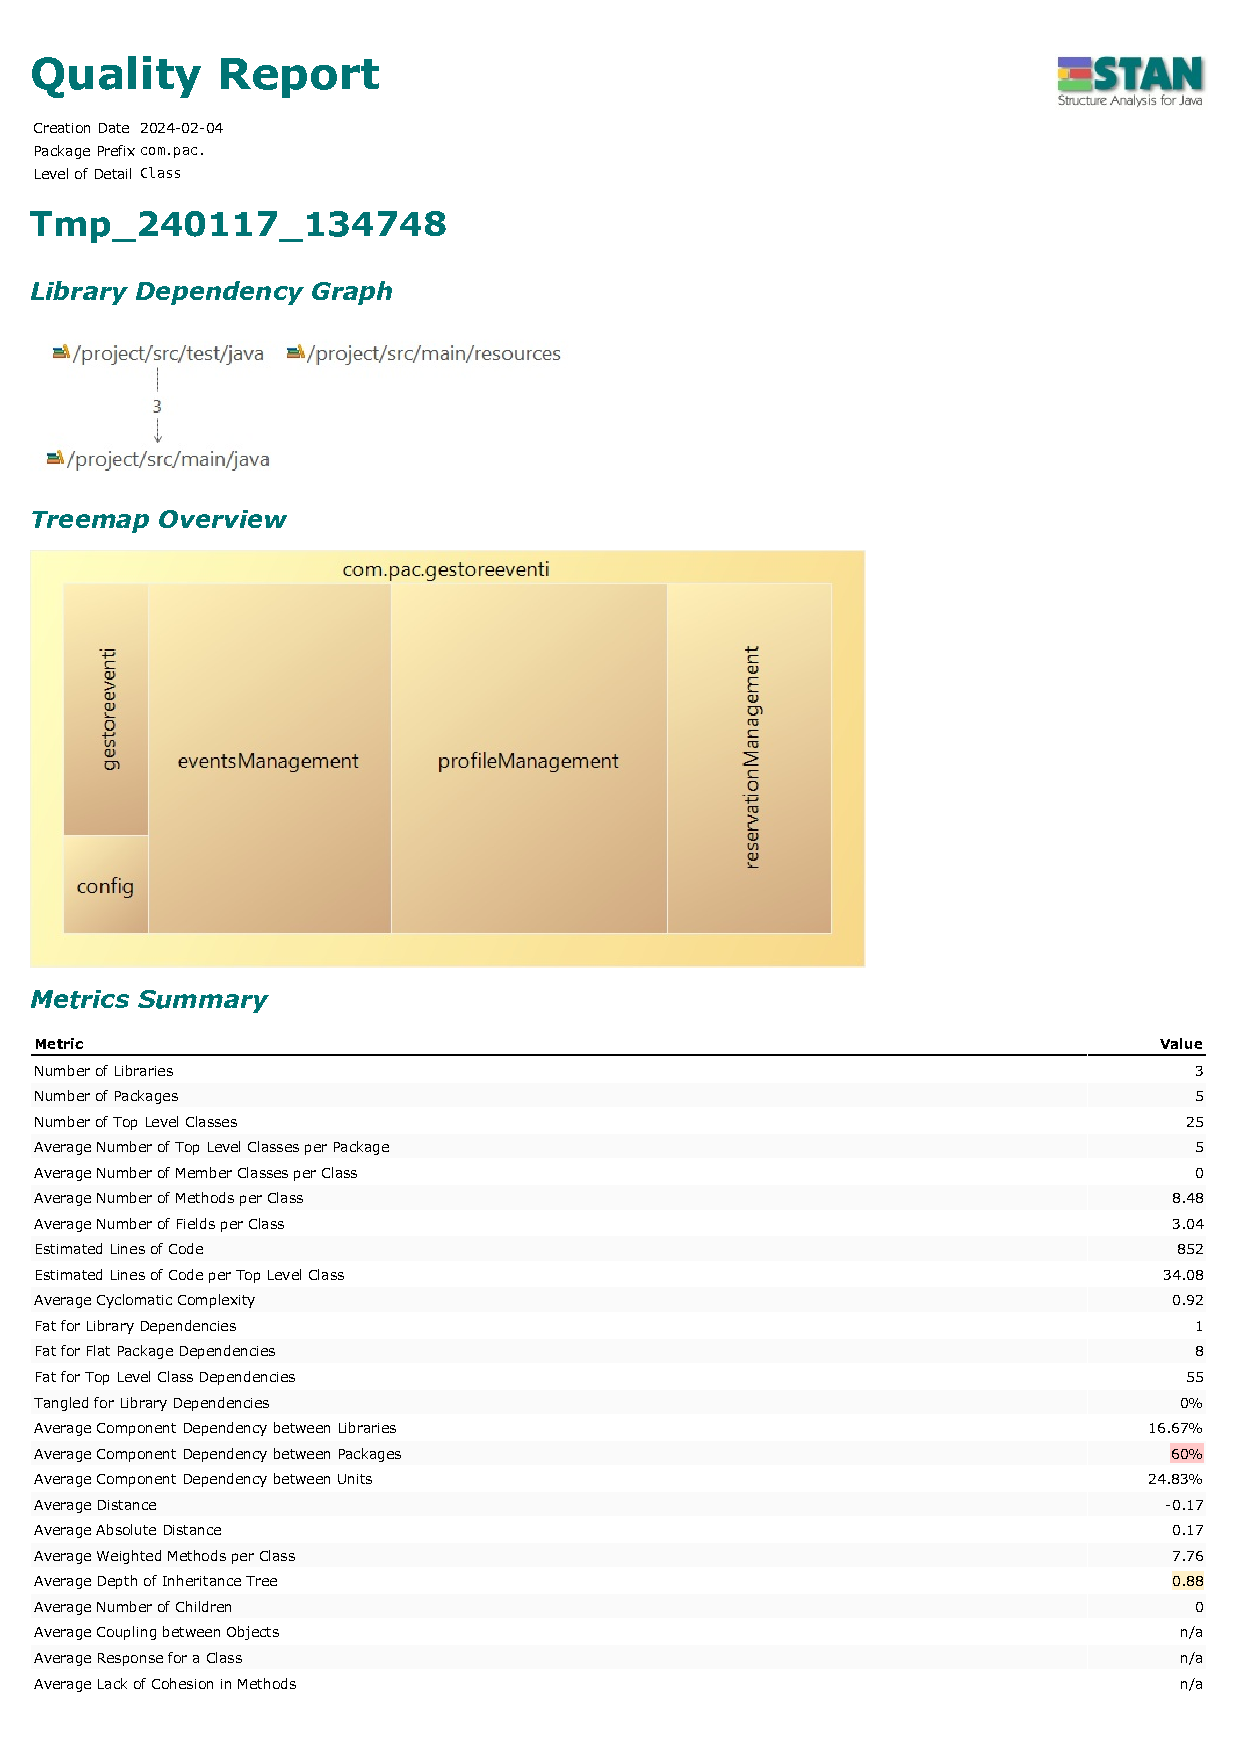
\includepdf[pages=-]{Iterazione 3/test/static analysis/static analysis.pdf}
\subsection{Analisi dinamica}
Nell’iterazione 3 sono state testate le seguenti API utilizzando Postman:
\begin{itemize}
	\item Visualizzazione del profilo di un utente;
	\item Visualizzazione del profilo di un organizzatore;
	\item Visualizzazione degli eventi consigliati all'utente;
  \item Visualizzazione dei dettagli di un evento;
  \item Visualizzazione delle informazioni meteorologiche;
  \item Visualizzazione degli utenti iscritti ad un evento;
\end{itemize}
\begin{figure}[h!]
\begin{center}
  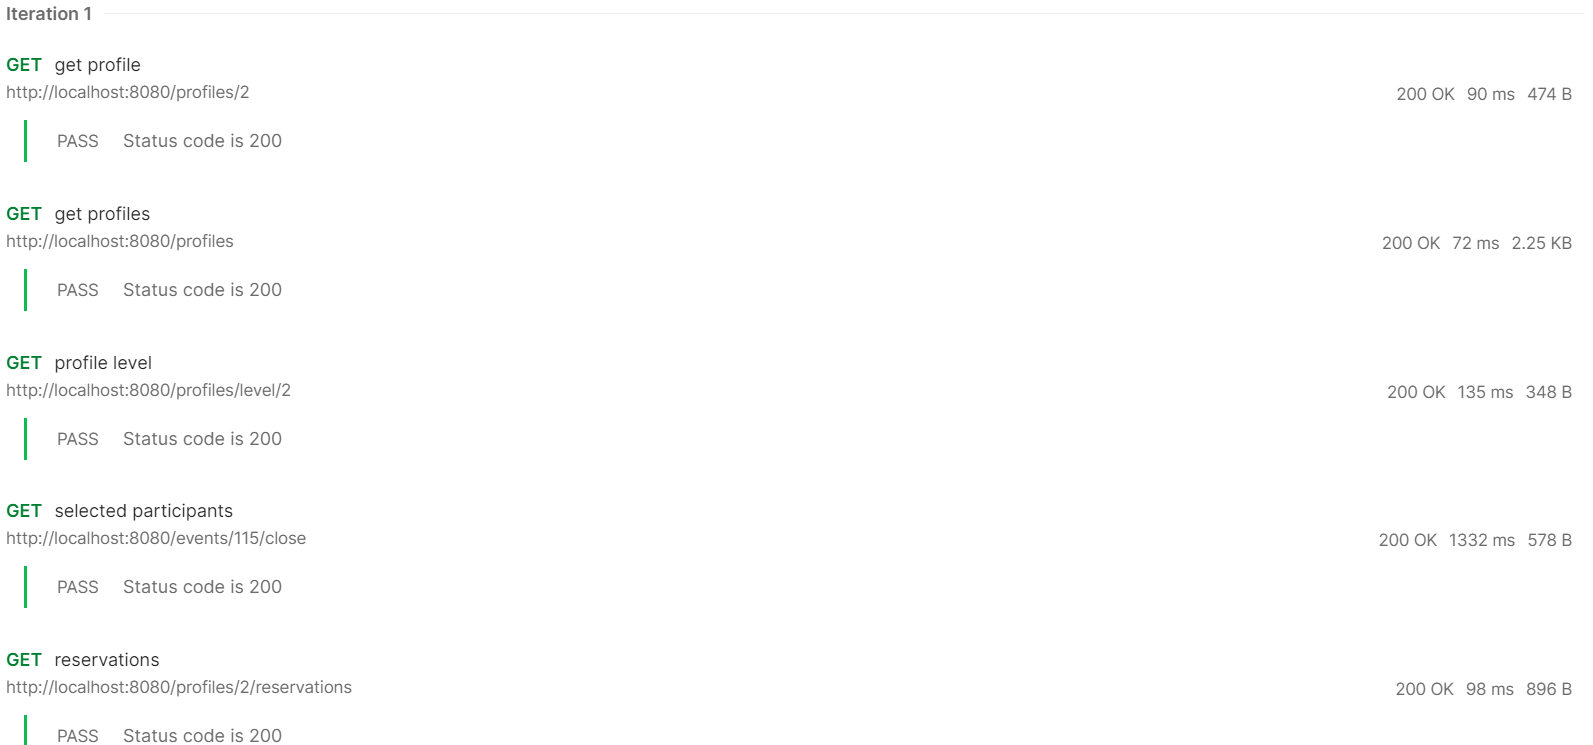
\includegraphics[width=1\textwidth]{Iterazione 3/images/it3_api.PNG}\\
  \caption{Test collection}
  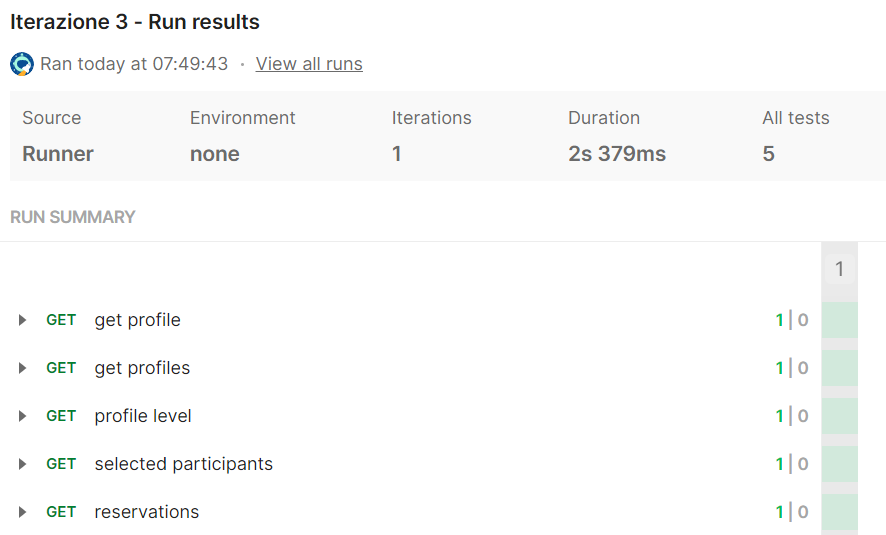
\includegraphics[width=1\textwidth]{Iterazione 3/images/it3.png}\\
\end{center}
\end{figure}
